\documentclass[11pt,a4paper]{article}

% Paquetes básicos
\usepackage[utf8]{inputenc}
\usepackage[T1]{fontenc}
\usepackage[spanish]{babel}
\usepackage{graphicx}
\usepackage{float}
\usepackage{amsmath}
\usepackage{listings}
\usepackage{xcolor}
\usepackage{booktabs}
\usepackage{subfig}

% Configuración de página y espaciado
\usepackage[left=2.5cm,right=2.5cm,top=3cm,bottom=3cm]{geometry}

% Ajuste específico para el TOC
\usepackage{tocloft}
\setlength{\cftbeforesecskip}{0.1pt}
\setlength{\cftbeforesubsecskip}{0.1pt}
\setlength{\cftbeforesubsubsecskip}{0.1pt}
\renewcommand{\cftsecfont}{\normalfont}
\renewcommand{\cftsecpagefont}{\normalfont}
\setlength{\cftparskip}{0pt}
\setlength{\cftbeforetoctitleskip}{0pt}
\setlength{\cftaftertoctitleskip}{0pt}

% Configuración de párrafos
\usepackage{parskip}
\setlength{\parindent}{0em}
\setlength{\parskip}{0.5em}

% Configuración de hyperref
\usepackage{hyperref}
\hypersetup{
	colorlinks=true,
	linkcolor=blue,
	filecolor=magenta,
	urlcolor=cyan,
	pdftitle={Práctica 2: Visión artificial y aprendizaje},
	pdfpagemode=FullScreen,
}

% Configuración de listings
\lstset{
	basicstyle=\ttfamily\small,
	breaklines=true,
	commentstyle=\color{green!60!black},
	keywordstyle=\color{blue},
	stringstyle=\color{red},
	numbers=left,
	numberstyle=\tiny\color{gray},
	numbersep=5pt,
	frame=single,
	backgroundcolor=\color{white}
}

% Control de profundidad del TOC
\setcounter{tocdepth}{2}
\setcounter{secnumdepth}{3}

\begin{document}
	
\begin{titlepage}
	\centering
	\vspace*{\fill}
	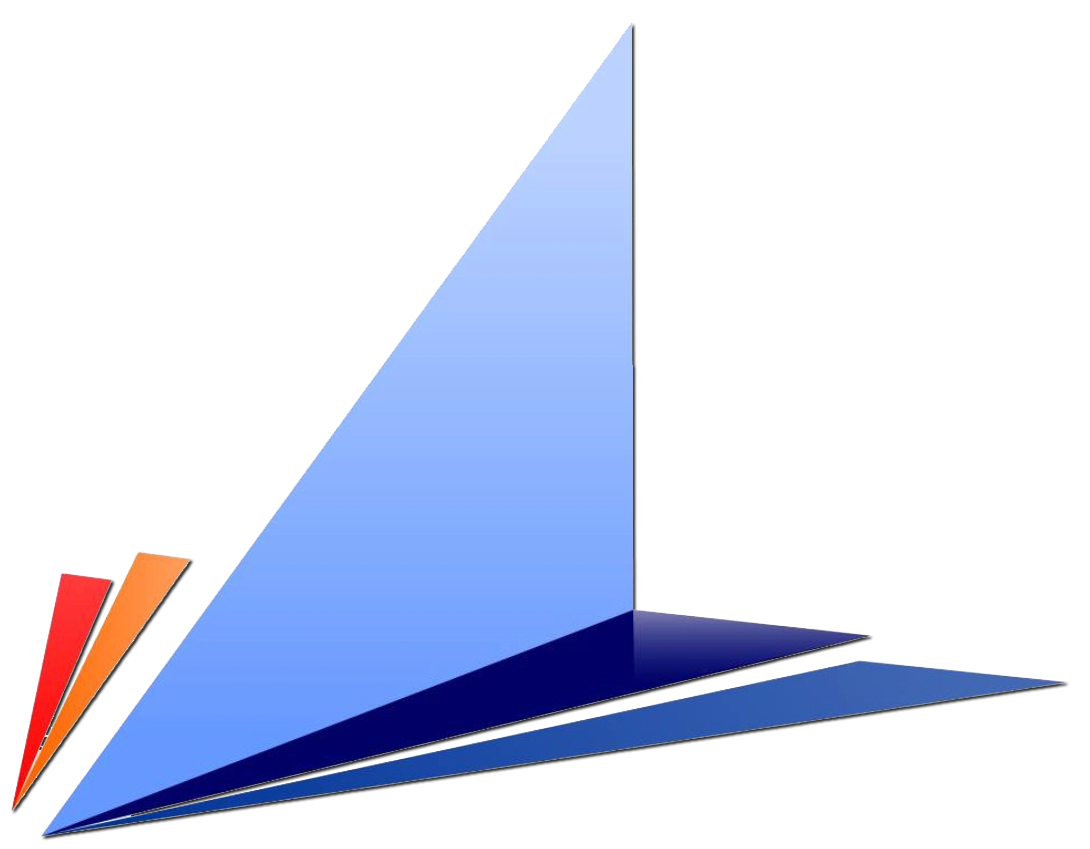
\includegraphics[width=0.2\textwidth]{logoeps}
	\vspace{1cm}
	{\bfseries Universidad de Alicante\par}
	\vspace{1cm}
	{\scshape\Large Ingeniería Informática\par}
	\vspace{2cm}
	{\scshape\Huge Sistemas Inteligentes\par}
	\vspace{2cm}
	{\itshape\Large Visión artificial y aprendizaje\par}
	\vspace{\fill}
	{\Large Autor:\par}
	{\Large Jaime Hernández Delgado (jhd3)\par}
	\vspace{\fill}
	{\Large Curso 2024/2025\par}
\end{titlepage}

\newpage

\tableofcontents
\newpage

\section{Introducción}
\subsection{Objetivos}

Esta práctica tiene como objetivo principal el desarrollo de capacidades en el ámbito del aprendizaje automático y la visión artificial, centrándose específicamente en la implementación y optimización de redes neuronales para la clasificación de imágenes. Los objetivos específicos son:

\begin{itemize}
    \item Comprender en profundidad el funcionamiento de las redes neuronales artificiales como técnicas de aprendizaje supervisado, con especial énfasis en:
    \begin{itemize}
        \item Perceptrones multicapa (MLP)
        \item Redes neuronales convolucionales (CNN)
    \end{itemize}

    \item Adquirir conocimientos fundamentales sobre el procesamiento de imágenes:
    \begin{itemize}
        \item Entender el concepto de imagen digital y píxel
        \item Comprender cómo las técnicas de aprendizaje supervisado pueden aplicarse para la clasificación de imágenes
    \end{itemize}

    \item Dominar el algoritmo de retropropagación (backpropagation) y sus componentes esenciales:
    \begin{itemize}
        \item Funciones de activación
        \item Optimizadores
        \item Funciones de pérdida
        \item Métricas de evaluación
    \end{itemize}

    \item Desarrollar habilidades prácticas en el uso de Keras:
    \begin{itemize}
        \item Implementación eficiente de redes neuronales
        \item Configuración y ajuste de hiperparámetros
        \item Evaluación de modelos
    \end{itemize}

    \item Aprender a optimizar el rendimiento de redes neuronales mediante:
    \begin{itemize}
        \item Ajuste del número de épocas de entrenamiento
        \item Configuración del tamaño de batch
        \item Selección de funciones de activación apropiadas
        \item Diseño de arquitecturas de red efectivas
    \end{itemize}

    \item Desarrollar competencias en visualización y análisis de resultados:
    \begin{itemize}
        \item Utilización de Matplotlib para la generación de gráficas
        \item Interpretación de métricas de rendimiento
        \item Análisis de matrices de confusión
    \end{itemize}

    \item Adquirir experiencia en la automatización de procesos:
    \begin{itemize}
        \item Desarrollo de scripts para pruebas automáticas
        \item Generación automatizada de resultados
        \item Creación eficiente de contenido para el informe
    \end{itemize}
\end{itemize}

A través de estos objetivos, se busca desarrollar una comprensión integral de las redes neuronales y su aplicación práctica en problemas de visión artificial, desde la implementación básica hasta la optimización avanzada de modelos.

\subsection{Herramientas y tecnologías utilizadas}

Para el desarrollo de esta práctica se han utilizado diversas herramientas y tecnologías del ecosistema de Python orientadas al aprendizaje automático y la ciencia de datos:

\subsubsection{Bibliotecaa principal}
\begin{itemize}
    \item \textbf{Keras}: API de alto nivel que se ejecuta sobre TensorFlow, que ofrece:
    \begin{itemize}
        \item Interfaz intuitiva para la construcción de redes neuronales
        \item Implementación rápida de modelos complejos
        \item Amplia variedad de capas predefinidas y funciones de activación
        \item Herramientas de preprocesamiento de datos
    \end{itemize}
\end{itemize}

\subsubsection{Bibliotecas de apoyo}
\begin{itemize}
    \item \textbf{NumPy}: Biblioteca fundamental para la computación científica en Python:
    \begin{itemize}
        \item Manipulación eficiente de arrays multidimensionales
        \item Operaciones matemáticas vectorizadas
        \item Funciones para el preprocesamiento de datos
    \end{itemize}
    
    \item \textbf{Matplotlib}: Biblioteca para la creación de visualizaciones:
    \begin{itemize}
        \item Generación de gráficas de evolución del entrenamiento
        \item Visualización de imágenes del dataset
        \item Creación de gráficas comparativas de resultados
    \end{itemize}
    
    \item \textbf{Seaborn}: Biblioteca de visualización estadística basada en Matplotlib:
    \begin{itemize}
        \item Generación de matrices de confusión
        \item Mejora visual de las gráficas estadísticas
    \end{itemize}
    
    \item \textbf{Scikit-learn}: Biblioteca para aprendizaje automático:
    \begin{itemize}
        \item Cálculo de métricas de evaluación
        \item Funciones de utilidad para el procesamiento de datos
    \end{itemize}
\end{itemize}

\subsubsection{Dataset}
\begin{itemize}
    \item \textbf{CIFAR-10}: Conjunto de datos estándar que contiene:
    \begin{itemize}
        \item 60.000 imágenes en color de 32x32 píxeles
        \item 10 clases diferentes (avión, automóvil, pájaro, gato, ciervo, perro, rana, caballo, barco y camión)
        \item 50.000 imágenes para entrenamiento y 10.000 para pruebas
        \item Distribución equilibrada de clases
    \end{itemize}
\end{itemize}

\subsubsection{Control de versiones y documentación}
\begin{itemize}
    \item \textbf{\LaTeX}: Sistema de composición de textos utilizado para la generación de esta memoria
    \item \textbf{Git}: Sistema de control de versiones para el seguimiento de cambios en el código
\end{itemize}

Todas estas herramientas y tecnologías han sido seleccionadas por su madurez, amplia documentación disponible y gran comunidad de usuarios, lo que facilita la resolución de problemas y el acceso a recursos de aprendizaje. Además, representan el estado del arte en el desarrollo de aplicaciones de aprendizaje automático y son ampliamente utilizadas tanto en entornos académicos como profesionales.

\newpage

\section{Desarrollo}

\subsection{Preprocesamiento de datos}

El preprocesamiento de los datos es un paso fundamental para el correcto funcionamiento de las redes neuronales. En esta práctica, trabajamos con el dataset CIFAR10, que requiere cierta preparación antes de poder ser utilizado efectivamente por nuestros modelos.

\subsubsection{Carga del dataset}
El primer paso consiste en cargar el dataset CIFAR10 utilizando las utilidades proporcionadas por Keras:

\begin{lstlisting}[language=Python]
(X_train, Y_train), (X_test, Y_test) = keras.datasets.cifar10.load_data()
\end{lstlisting}

Tras la carga inicial, los datos presentan las siguientes características:
\begin{itemize}
    \item \textbf{X\_train}: Array de 50.000 imágenes de entrenamiento de dimensiones (32, 32, 3)
    \item \textbf{Y\_train}: Array de 50.000 etiquetas de entrenamiento
    \item \textbf{X\_test}: Array de 10.000 imágenes de prueba de dimensiones (32, 32, 3)
    \item \textbf{Y\_test}: Array de 10.000 etiquetas de prueba
\end{itemize}

\subsubsection{Normalización de las imágenes}
Las imágenes originales tienen valores de píxeles en el rango [0, 255]. Para mejorar el entrenamiento de las redes neuronales, es necesario normalizar estos valores al rango [0, 1]:

\begin{lstlisting}[language=Python]
X_train = X_train.astype('float32') / 255.0
X_test = X_test.astype('float32') / 255.0
\end{lstlisting}

Esta normalización es importante por varios motivos:
\begin{itemize}
    \item Evita problemas de escala en los cálculos numéricos
    \item Ayuda a que el proceso de entrenamiento sea más estable
    \item Facilita la convergencia del algoritmo de optimización
\end{itemize}

\subsubsection{Preprocesamiento específico para MLP}
Para las redes neuronales tipo MLP, es necesario aplanar las imágenes ya que estas redes esperan datos de entrada unidimensionales:

\begin{lstlisting}[language=Python]
X_train_mlp = X_train.reshape((X_train.shape[0], -1))  # (50000, 3072)
X_test_mlp = X_test.reshape((X_test.shape[0], -1))     # (10000, 3072)
\end{lstlisting}

Esta transformación convierte cada imagen de una matriz 32x32x3 en un vector de 3.072 elementos (32 * 32 * 3).

\subsubsection{Codificación de etiquetas}
Las etiquetas originales están en formato de índice (números del 0 al 9). Para el entrenamiento, necesitamos convertirlas a formato one-hot encoding:

\begin{lstlisting}[language=Python]
Y_train = keras.utils.to_categorical(Y_train, 10)
Y_test = keras.utils.to_categorical(Y_test, 10)
\end{lstlisting}

Esta transformación convierte cada etiqueta en un vector de 10 elementos donde:
\begin{itemize}
    \item El valor 1 indica la clase correcta
    \item El resto de valores son 0
    \item Por ejemplo, la clase 3 se convierte en [0, 0, 0, 1, 0, 0, 0, 0, 0, 0]
\end{itemize}

\subsubsection{Consideraciones para CNN}
Para las redes neuronales convolucionales (CNN), no es necesario aplanar las imágenes, ya que estas redes están diseñadas para trabajar directamente con datos bidimensionales. Por lo tanto, mantendremos la estructura original de las imágenes (32, 32, 3) cuando trabajemos con CNNs.

\subsubsection{Validación de los datos}
Después del preprocesamiento, es importante verificar:
\begin{itemize}
    \item Que los valores de los píxeles estén en el rango [0, 1]
    \item Que las dimensiones de los arrays sean correctas
    \item Que las etiquetas estén correctamente codificadas
\end{itemize}

\begin{lstlisting}[language=Python]
print(f"Rango de valores X_train: [{X_train.min()}, {X_train.max()}]")
print(f"Forma X_train MLP: {X_train_mlp.shape}")
print(f"Forma Y_train: {Y_train.shape}")
\end{lstlisting}

Este preprocesamiento es crucial para el correcto funcionamiento de nuestros modelos y nos permitirá obtener mejores resultados durante el entrenamiento.

\subsection{Tarea A: Implementación básica de MLP}

\subsubsection{Fundamentos teóricos}

El Perceptrón Multicapa (Multi-Layer Perceptron, MLP) es una de las arquitecturas más fundamentales de redes neuronales artificiales. Se compone de múltiples capas de neuronas artificiales organizadas de manera jerárquica, donde cada neurona en una capa está conectada con todas las neuronas de la capa siguiente.

\paragraph{Estructura básica:}
Un MLP típico consta de tres tipos principales de capas:
\begin{itemize}
    \item \textbf{Capa de entrada}: Recibe los datos de entrada (en nuestro caso, los píxeles de la imagen)
    \item \textbf{Capas ocultas}: Realizan transformaciones no lineales de los datos
    \item \textbf{Capa de salida}: Produce la predicción final (en nuestro caso, la clasificación de la imagen)
\end{itemize}

\paragraph{Funcionamiento:}
El proceso de una neurona artificial se puede describir matemáticamente como:
\[ y = f(\sum_{i=1}^{n} w_i x_i + b) \]
Donde:
\begin{itemize}
    \item $x_i$ son las entradas
    \item $w_i$ son los pesos asociados a cada entrada
    \item $b$ es el sesgo (bias)
    \item $f$ es la función de activación
    \item $y$ es la salida de la neurona
\end{itemize}

\paragraph{Función de activación:}
En nuestra implementación inicial utilizamos la función sigmoid para las capas ocultas:
\[ sigmoid(x) = \frac{1}{1 + e^{-x}} \]
Y softmax para la capa de salida:
\[ softmax(x_i) = \frac{e^{x_i}}{\sum_{j=1}^{n} e^{x_j}} \]

\paragraph{Proceso de aprendizaje:}
El aprendizaje en un MLP ocurre mediante el algoritmo de retropropagación (backpropagation):
\begin{enumerate}
    \item \textbf{Propagación hacia adelante}: Los datos atraviesan la red, generando una predicción
    \item \textbf{Cálculo del error}: Se compara la predicción con el valor real
    \item \textbf{Retropropagación}: El error se propaga hacia atrás en la red
    \item \textbf{Actualización de pesos}: Se ajustan los pesos para minimizar el error
\end{enumerate}

\subsection{Tarea B: Ajuste del número de épocas}

\subsubsection{Fundamentos teóricos}
En el contexto del aprendizaje automático, una época representa una pasada completa a través de todo el conjunto de datos de entrenamiento. El número de épocas es un hiperparámetro crucial que determina cuántas veces el algoritmo procesará el conjunto de datos completo durante el entrenamiento.

El sobreentrenamiento (overfitting) es un fenómeno que ocurre cuando un modelo aprende con demasiado detalle los datos de entrenamiento, hasta el punto de memorizar sus particularidades y ruido, en lugar de aprender patrones generales. Esto resulta en:

\begin{itemize}
	\item Un rendimiento excelente en los datos de entrenamiento
	\item Un rendimiento deficiente en datos nuevos (baja capacidad de generalización)
	\item Una brecha creciente entre el rendimiento en entrenamiento y validación
\end{itemize}

La relación entre el número de épocas y el sobreentrenamiento es directa:
\begin{itemize}
	\item Pocas épocas pueden resultar en subentrenamiento (underfitting), donde el modelo no ha aprendido suficientemente los patrones de los datos
	\item Demasiadas épocas pueden llevar al sobreentrenamiento, donde el modelo memoriza los datos de entrenamiento
	\item El desafío está en encontrar el punto óptimo entre estos dos extremos
\end{itemize}

\subsubsection{Experimentación}
Para encontrar el número óptimo de épocas, se realizaron experimentos con diferentes configuraciones:

\paragraph{Configuración del experimento:}
\begin{itemize}
	\item Valores de épocas probados: [5, 10, 20, 50, 100]
	\item Arquitectura del modelo: MLP con una capa oculta de 32 neuronas
	\item Función de activación: sigmoid en la capa oculta, softmax en la capa de salida
	\item Optimizador: Adam
	\item División de datos: 90\% entrenamiento, 10\% validación
\end{itemize}

\paragraph{Métricas monitorizadas:}
\begin{itemize}
	\item Precisión (accuracy) en entrenamiento y validación
	\item Tiempo de entrenamiento
	\item Pérdida (loss) en entrenamiento y validación
\end{itemize}

\subsubsection{Resultados y análisis}

\paragraph{Análisis de la precisión:}
La precisión del modelo evoluciona de la siguiente manera:
\begin{itemize}
	\item 5 épocas: 0.39 (insuficiente entrenamiento)
	\item 20 épocas: 0.43 (mejora significativa)
	\item 50 épocas: 0.453 (mejor rendimiento)
	\item 100 épocas: 0.44 (ligera degradación)
\end{itemize}

\begin{figure}[H]
	\centering
	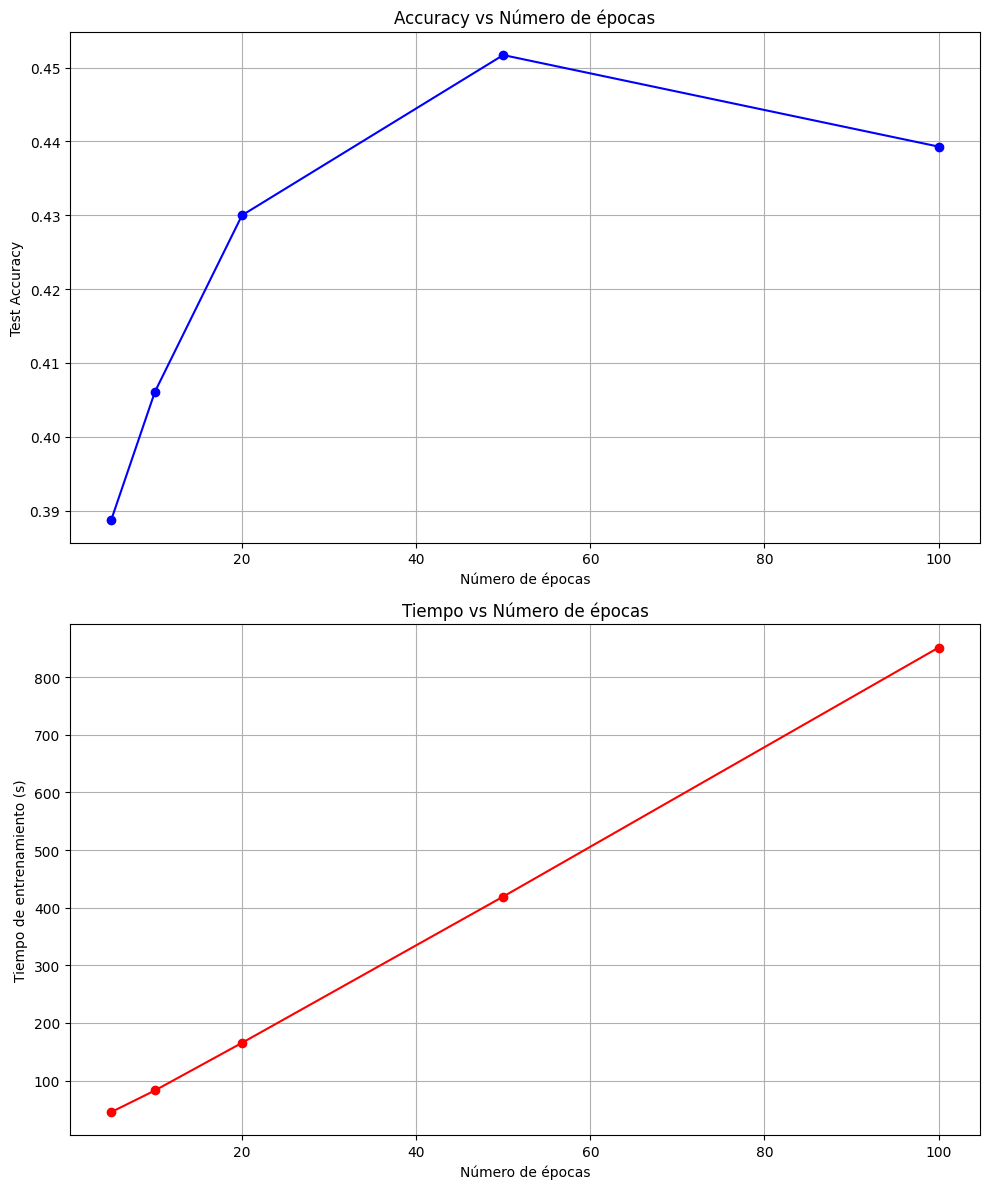
\includegraphics[width=0.8\textwidth]{images/accuracy_vs_epocas}
	\caption{Evolución de la precisión según el número de épocas}
	\label{fig:accuracy_epocas}
\end{figure}

\paragraph{Análisis del coste computacional:}
El tiempo de entrenamiento muestra una relación lineal con el número de épocas:
\begin{itemize}
	\item 5 épocas: $\approx$ 50 segundos
	\item 50 épocas: $\approx$ 400 segundos
	\item 100 épocas: $\approx$ 800 segundos
\end{itemize}

\paragraph{Análisis de las curvas de aprendizaje:}
Las curvas de aprendizaje del mejor modelo (50 épocas) revelan:
\begin{itemize}
	\item Una mejora constante en la precisión de entrenamiento hasta alcanzar 0.50
	\item Una estabilización de la precisión de validación alrededor de 0.43-0.45
	\item Una brecha creciente entre entrenamiento y validación, indicando inicio de sobreentrenamiento
\end{itemize}

\begin{figure}[H]
	\centering
	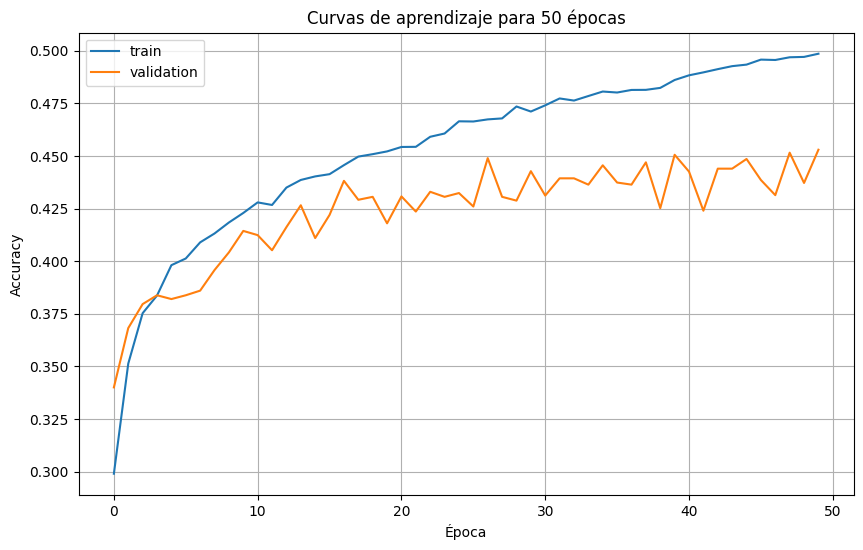
\includegraphics[width=0.8\textwidth]{images/curvas_aprendizaje}
	\caption{Curvas de aprendizaje para el modelo de 50 épocas}
	\label{fig:curvas_aprendizaje}
\end{figure}

\paragraph{Conclusiones:}
\begin{itemize}
	\item El número óptimo de épocas para este modelo es 50, proporcionando el mejor balance entre precisión y tiempo de entrenamiento
	\item Entrenar más allá de 50 épocas resulta en:
	\begin{itemize}
		\item Mayor tiempo de computación
		\item Inicio de sobreentrenamiento
		\item Degradación de la capacidad de generalización
	\end{itemize}
	\item Se observa una clara relación entre el número de épocas y el riesgo de sobreentrenamiento
\end{itemize}

\paragraph{Recomendaciones:}
\begin{itemize}
	\item Utilizar 50 épocas como valor de referencia para futuros experimentos
	\item Considerar la implementación de técnicas de regularización para reducir el sobreentrenamiento
	\item Implementar early stopping para optimizar automáticamente el tiempo de entrenamiento
\end{itemize}

\subsection{Tarea C: Ajuste del tamaño de batch}
% Misma estructura que las anteriores
\subsubsection{Fundamentos teóricos}
% Explicar qué es el sobreentrenamiento y su relación con las épocas

\subsubsection{Experimentación}
% Describir los experimentos realizados

\subsubsection{Resultados y análisis}
% Mostrar y analizar los resultados

\subsection{Tarea D: Funciones de activación}
% Misma estructura que las anteriores
\subsubsection{Fundamentos teóricos}
% Explicar qué es el sobreentrenamiento y su relación con las épocas

\subsubsection{Experimentación}
% Describir los experimentos realizados

\subsubsection{Resultados y análisis}
% Mostrar y analizar los resultados

\subsection{Tarea E: Ajuste del número de neuronas}
% Misma estructura que las anteriores
\subsubsection{Fundamentos teóricos}
% Explicar qué es el sobreentrenamiento y su relación con las épocas

\subsubsection{Experimentación}
% Describir los experimentos realizados

\subsubsection{Resultados y análisis}
% Mostrar y analizar los resultados

\subsection{Tarea F: Optimización de MLP multicapa}
% Misma estructura que las anteriores
\subsubsection{Fundamentos teóricos}
% Explicar qué es el sobreentrenamiento y su relación con las épocas

\subsubsection{Experimentación}
% Describir los experimentos realizados

\subsubsection{Resultados y análisis}
% Mostrar y analizar los resultados

\subsection{Tarea G: Implementación de CNN}
% Misma estructura que las anteriores
\subsubsection{Fundamentos teóricos}
% Explicar qué es el sobreentrenamiento y su relación con las épocas

\subsubsection{Experimentación}
% Describir los experimentos realizados

\subsubsection{Resultados y análisis}
% Mostrar y analizar los resultados

\subsection{Tarea H: Ajuste del tamaño de kernel}
% Misma estructura que las anteriores
\subsubsection{Fundamentos teóricos}
% Explicar qué es el sobreentrenamiento y su relación con las épocas

\subsubsection{Experimentación}
% Describir los experimentos realizados

\subsubsection{Resultados y análisis}
% Mostrar y analizar los resultados

\subsection{Tarea I: Optimización de la arquitectura CNN}
% Misma estructura que las anteriores
\subsubsection{Fundamentos teóricos}
% Explicar qué es el sobreentrenamiento y su relación con las épocas

\subsubsection{Experimentación}
% Describir los experimentos realizados

\subsubsection{Resultados y análisis}
% Mostrar y analizar los resultados

\section{Conclusiones}
% Resumen de los resultados más importantes y lecciones aprendidas

\section{Bibliografía}
\begin{thebibliography}{9}
    \bibitem{keras} Keras documentation, \url{https://keras.io/}
    % Añadir el resto de referencias utilizadas
\end{thebibliography}

\appendix
\section{Anexos}
% Aquí puedes incluir código fuente completo, resultados adicionales, etc.

\end{document}